% =====================================================================
%  HATI v2.5 -- Shadow Kinematics: a solar-sweep sub-resolution channel
%  Author: Gergő Csaba Morvai
%  Engine: LuaLaTeX  (compile: latexmk -lualatex shadow_kinematics.tex)
%  Bibliography: biblatex + biber
% =====================================================================
\documentclass[11pt]{article}

\usepackage{fontspec}
\usepackage{microtype}
\usepackage[a4paper,margin=2.45cm]{geometry}
\usepackage{graphicx}
\graphicspath{{../output/athena/}{../data/lroc_published/}{../output/}}
\usepackage{amsmath,amssymb}
\usepackage{xcolor}
\usepackage{booktabs}
\usepackage{array}
\usepackage{siunitx}
\usepackage[font=small]{caption}
\usepackage{enumitem}
\usepackage{tikz}
\usetikzlibrary{positioning,arrows.meta,calc,shapes.geometric,backgrounds,fit,decorations.pathmorphing}
\usepackage{tcolorbox}
\tcbuselibrary{skins,breakable}
\usepackage{titlesec}
\usepackage[backend=biber,style=authoryear,sorting=nyt,maxcitenames=2,uniquelist=false]{biblatex}
\addbibresource{references.bib}
\usepackage[hidelinks]{hyperref}
\usepackage{cleveref}

\setmainfont{TeX Gyre Pagella}
\setsansfont{TeX Gyre Heros}[Scale=0.92]
\setmonofont{TeX Gyre Cursor}[Scale=0.90]

\definecolor{hatiblue}{HTML}{1F3A5F}
\definecolor{hatiaccent}{HTML}{B23A2E}
\definecolor{hatiteal}{HTML}{1B7A6E}
\definecolor{hatipurple}{HTML}{5B4B8A}
\definecolor{plainbg}{HTML}{EAF2FB}
\definecolor{plainframe}{HTML}{2E6DB4}
\definecolor{intentbg}{HTML}{F0EEF6}
\definecolor{intentframe}{HTML}{5B4B8A}
\definecolor{limitbg}{HTML}{FBEEEC}
\definecolor{limitframe}{HTML}{B23A2E}

\titleformat{\section}{\sffamily\Large\bfseries\color{hatiblue}}{\thesection}{0.6em}{}
\titleformat{\subsection}{\sffamily\large\bfseries\color{hatiblue!88}}{\thesubsection}{0.5em}{}
\titleformat{\subsubsection}{\sffamily\normalsize\bfseries\color{hatiaccent}}{}{0em}{}
\titlespacing*{\section}{0pt}{1.6ex plus .3ex}{0.8ex}

\newtcolorbox{plainbox}{breakable,enhanced,colback=plainbg,colframe=plainframe,
  boxrule=0.6pt,arc=2pt,left=7pt,right=7pt,top=4pt,bottom=4pt,
  fonttitle=\bfseries\sffamily\small,coltitle=plainframe,
  attach boxed title to top left={xshift=8pt,yshift=-7pt},
  boxed title style={colback=plainbg,colframe=plainframe,boxrule=0.4pt,arc=1pt},
  title={In plain words}}
\newtcolorbox{intentbox}{breakable,enhanced,colback=intentbg,colframe=intentframe,
  boxrule=0.6pt,arc=2pt,left=7pt,right=7pt,top=4pt,bottom=4pt,
  fonttitle=\bfseries\sffamily\small,coltitle=intentframe,
  attach boxed title to top left={xshift=8pt,yshift=-7pt},
  boxed title style={colback=intentbg,colframe=intentframe,boxrule=0.4pt,arc=1pt},
  title={Why it is built this way}}
\newtcolorbox{limitbox}{breakable,enhanced,colback=limitbg,colframe=limitframe,
  boxrule=0.6pt,arc=2pt,left=7pt,right=7pt,top=4pt,bottom=4pt,
  fonttitle=\bfseries\sffamily\small,coltitle=limitframe,
  attach boxed title to top left={xshift=8pt,yshift=-7pt},
  boxed title style={colback=limitbg,colframe=limitframe,boxrule=0.4pt,arc=1pt},
  title={Honest limit}}

\sisetup{detect-all,per-mode=symbol}
\DeclareSIUnit{\px}{px}
\setlist{nosep,leftmargin=1.4em}
\captionsetup{labelfont={bf,sf,color=hatiblue}}

% =====================================================================
\title{\sffamily\bfseries\color{hatiblue}\LARGE Shadow Kinematics\\[3pt]
\Large\mdseries Using the Sun's motion to turn a solar sweep into a\\ sub-resolution lunar hazard map}
\author{\large Gergő Csaba Morvai\\[2pt]
\normalsize\itshape HATI v2.5 \textendash{} M\'ani Mission terrain-hazard pipeline}
\date{\normalsize June 2026}

\begin{document}
\maketitle

\begin{abstract}
\noindent
A lander is endangered by obstacles smaller than the elevation models used to choose
where it sets down. HATI's roughness heatmap and deterministic slope gate work on those
elevation models, so they are blind by construction to a metre-scale boulder or a shallow
few-metre crater --- exactly the class of hazard tied to the 2025 IM-2 ``Athena'' upset.
A single shadow photograph reaches below the elevation floor, but on its own it cannot
tell a real shadow from a patch of dark rock, cannot fix an obstacle's sign or height
without assuming the ground is flat, and only ever sees the obstacles that happen to throw
a shadow toward the camera under that one Sun. This note develops a channel that removes
all three limitations at once by treating the Sun as a moving probe. Over a \emph{solar
sweep} --- many orthophotos of one site under different solar azimuths --- a true obstacle
casts a shadow that pivots around a fixed base, while a dark albedo mark does not move.
Accumulating one vote at the up-Sun base of every detected shadow makes a real obstacle's
votes \emph{converge} into a sharp confidence peak whose statistics give its height, while
an albedo decoy's votes \emph{smear} into a ring and self-cancel. We give the forward
model, the voting estimator, and a synthetic ground-truth benchmark: across a
\SIrange{0}{360}{\degree} sweep at \ang{5} solar elevation, the detector recovers the
heights of \SIrange{0.3}{3}{\meter} obstacles --- well below the elevation-model floor ---
to an RMS error of \SI{0.24}{\meter}, holds detection AUC at \num{0.99}, and drives the
confidence of albedo decoys to zero (a signal-to-decoy separation of $\sim$\num{8000}). A
query of the public archive shows the sweep is not hypothetical: \num{696} narrow-angle
frames already cover the Athena site, \num{525} with the Sun up and all twelve azimuth
sectors filled. We state plainly what the synthetic benchmark does and does not establish,
and fence the real-data step that remains.
\end{abstract}

\noindent\textbf{\sffamily\color{hatiblue}Keywords:}\enspace lunar landing hazards;
shadow photoclinometry; multi-illumination; solar sweep; sub-resolution obstacles; LROC NAC; Mons Mouton.

\medskip\hrule\medskip

% =====================================================================
\section{The gap this channel fills}

HATI carries two elevation-model channels: a multi-scale roughness heatmap and, in v2.5, a
deterministic gate that flags ground whose footprint-scale slope or relief exceeds a stated
lander limit, in physical units \autocite{henriksen2017}. Both inherit the resolution of
the elevation model they read. For the south-polar Mons Mouton site that means a
\SI{4}{\meter} posting and an effective resolution near \SIrange{16}{19}{\meter} once noise
is accounted for. At that scale the Athena touchdown is benign: the footprint slope is a
gentle \ang{2.8} and the gate passes it. The hazard the Lunar Reconnaissance Orbiter Camera
(LROC) team tied to the upset --- a crater roughly \SI{20}{\meter} across on slightly sloped
ground --- lives at or below the elevation model's floor. No amount of re-weighting an
elevation channel recovers a feature the elevation model never resolved.

The shadow census in HATI v2.0 was the first reach below that floor: a single orthophoto at
\SI{0.9}{\meter} per pixel \autocite{robinson2010} resolves the \emph{shadow} a sub-floor
obstacle throws, because a shadow is geometrically amplified. At a solar elevation $e$, an
object of height $h$ casts a shadow of length
\begin{equation}
  L \;=\; h\,\cot e .
  \label{eq:shadowlaw}
\end{equation}
At the pole the Sun never climbs above $\sim$\ang{7}, so $\cot e$ runs from about \num{8} to
\num{30}: a \SI{0.3}{\meter} rock --- a third of a pixel, invisible in elevation --- lays
down a \SIrange{3}{6}{\meter} shadow spanning several pixels. The geometry does the
super-resolution for free.

But one photograph carries three intrinsic weaknesses. A dark patch of low-reflectance
rock looks just like a shadow to a single-frame threshold. The same shadow length implies a
different height depending on the unknown slope the shadow falls across. And a given frame
only shadows the obstacles oriented to cast toward the camera under that one Sun, so its
recall is hostage to the lighting it happened to get. The channel developed here keeps the
sub-floor reach of the shadow and removes all three weaknesses by letting the Sun move.

\begin{plainbox}
An elevation map can only warn you about bumps it is sharp enough to see. A shadow in a
photograph is the giveaway of a bump far too small for the map --- a pebble at dawn throws a
long shadow. The trouble is that a single photo can confuse a real pebble's shadow with a
dark smear of paint, and cannot measure how tall the pebble is. The fix is to watch the
same ground through a whole lunar day: a real bump's shadow swings around it like a sundial,
a smear of paint just sits there. Follow the swing and you confirm the bump and measure its
height.
\end{plainbox}

% =====================================================================
\section{Principle: the Sun as a moving probe}

Consider a fixed obstacle at ground position $\mathbf{x}_0$. Under a Sun at azimuth
$\varphi$ and elevation $e$, it shadows the ground in the anti-solar direction, starting at
its own base $\mathbf{x}_0$ and extending a distance $L=h\cot e$. Two facts follow, and they
are the whole method.

\emph{The base is invariant; the shadow is not.} As $\varphi$ sweeps through a lunar day,
the shadow rotates about $\mathbf{x}_0$ and changes length with $e$, but the end anchored at
the obstacle stays put. The \emph{up-Sun extreme} of the cast shadow --- its end nearest the
Sun --- is therefore an estimator of $\mathbf{x}_0$ that every frame agrees on.

\emph{Albedo does not move.} A patch of dark rock is dark because of what it is made of, not
where the Sun is. Its darkness neither rotates nor lengthens with $\varphi$. Whatever
``up-Sun extreme'' a detector assigns it slides around its own rim as the Sun circles, never
settling on one point.

These two facts separate topography from paint without any reflectance model. We turn them
into a map by accumulation.

\begin{intentbox}
We deliberately avoid inverting a photometric model pixel-by-pixel, which would need an
accurate lunar reflectance law \autocite{hapke1984,sato2014} and clean radiometric
cross-calibration between frames taken years apart. The voting estimator below asks only a
\emph{geometric} question --- does the up-Sun end of this shadow sit in the same place every
time the Sun moves? --- which is robust to the very calibration errors that would sink a
photometric inversion, and which a flight reviewer can audit.
\end{intentbox}

% =====================================================================
\section{The estimator}

Let the sweep be $K$ co-registered orthophotos, frame $k$ taken under $(\varphi_k,e_k)$. In
each frame we detect shadow pixels by a local-relative threshold --- a pixel is in shadow if
its brightness falls below half of the local sunlit background, estimated by a wide
separable mean --- and group them into connected regions. For a region $R$ we form two
projections onto the in-plane unit vector $\hat{\mathbf{s}}_k$ pointing toward the Sun and
its perpendicular $\hat{\mathbf{s}}_k^{\perp}$:
\begin{equation}
  \ell_{\parallel}(R)=\operatorname{ptp}_{\,p\in R}\langle p,\hat{\mathbf{s}}_k\rangle,
  \qquad
  \ell_{\perp}(R)=\operatorname{ptp}_{\,p\in R}\langle p,\hat{\mathbf{s}}_k^{\perp}\rangle ,
\end{equation}
where $\operatorname{ptp}$ is the peak-to-peak extent in metres. A cast shadow is elongated
along the anti-solar axis, so we keep only regions with
\begin{equation}
  \ell_{\parallel}(R)\;\ge\;1.8\,\max\!\big(\ell_{\perp}(R),\,\Delta\big),
  \label{eq:gate}
\end{equation}
$\Delta$ being the pixel size. This \emph{orientation gate} discards round dark blobs in any
single frame; the streaks it lets through are handled by the accumulation. For each
surviving region we read off the caster base and a height estimate,
\begin{equation}
  \mathbf{b}_R=\arg\max_{p\in R}\langle p,\hat{\mathbf{s}}_k\rangle,
  \qquad
  \hat h_R=\ell_{\parallel}(R)\,\tan e_k ,
  \label{eq:vote}
\end{equation}
the second line being \cref{eq:shadowlaw} solved for $h$. We then cast one vote into two
accumulators on the common grid,
\begin{equation}
  E(\mathbf{b}_R)\mathrel{+}=1,
  \qquad
  H(\mathbf{b}_R)\mathrel{+}=\hat h_R .
\end{equation}
After the sweep, the obstacle confidence and height maps are
\begin{equation}
  C=G_{\sigma}\!*E,
  \qquad
  \widehat{h}(\mathbf{x})=\frac{H(\mathbf{x})}{\max\!\big(E(\mathbf{x}),1\big)} ,
  \label{eq:maps}
\end{equation}
with $G_\sigma$ a small Gaussian that lets votes within a footprint reinforce.

The separation is now visible in $C$. For a true obstacle, $\mathbf{b}_R\!\approx\!\mathbf{x}_0$
for all $k$, so $E$ piles $K$ votes onto one cell and $C$ shows a sharp peak; the spread of
the $\hat h_R$ about a single value is the height. For an albedo feature, $\mathbf{b}_R$
walks around the patch rim as $\varphi_k$ turns, so the same $K$ detections scatter over an
annulus, $E$ stays low everywhere, and $C$ never peaks. Convergence is the signature of
topography; smear is the signature of paint.

% =====================================================================
\section{A ground-truth benchmark}

Because the real on-site sweep is not yet co-registered (\cref{sec:limits}), we validate the
estimator where the truth is known exactly. We build a synthetic scene at the orthophoto's
\SI{0.9}{\meter} pixel: \num{70} obstacles of height \SIrange{0.3}{3}{\meter} with footprints
of one-to-two pixels --- that is, \SIrange{0.9}{1.8}{\meter}, below the elevation-model floor
--- scattered on flat ground, together with \num{40} deliberately adversarial decoys: round
low-albedo patches and \emph{fixed dark streaks} that mimic an elongated shadow in any one
frame. Each frame is rendered by ray-marching the true cast shadow of the height field under
a chosen $(\varphi,e)$ at \ang{5} elevation, with read noise added. We run the estimator on
sweeps of $1,3,6,12,24$ and \num{48} azimuths evenly spaced over \SIrange{0}{360}{\degree},
and score the confidence map against the known obstacle positions.

\begin{table}[h]
\centering\small
\caption{Synthetic-sweep benchmark. Detection AUC saturates early --- the orientation gate
alone rejects round decoys in one frame --- but the quantities a single image cannot provide
improve monotonically with the sweep: obstacle confidence climbs while decoy confidence
stays at zero, and heights are recovered to a quarter of a metre.}
\label{tab:bench}
\begin{tabular}{rccccc}
\toprule
frames & azimuths & detection AUC & decoy conf. & obstacle conf. & height RMSE \\
\midrule
1  & 1  & 0.956 & 0.00 & 0.02 & \SI{0.20}{\meter} \\
3  & 3  & 0.988 & 0.00 & 0.07 & \SI{0.23}{\meter} \\
6  & 6  & 0.989 & 0.00 & 0.15 & \SI{0.23}{\meter} \\
12 & 12 & 0.990 & 0.00 & 0.30 & \SI{0.21}{\meter} \\
24 & 24 & 0.990 & 0.00 & 0.52 & \SI{0.23}{\meter} \\
48 & 48 & 0.990 & 0.00 & 1.08 & \SI{0.24}{\meter} \\
\bottomrule
\end{tabular}
\end{table}

\Cref{tab:bench} and \cref{fig:bench} carry the result. It would be dishonest to sell this on
the detection AUC, which is already \num{0.956} from a single frame --- the orientation gate
of \cref{eq:gate} does most of that work by itself, because a round albedo blob is not
elongated along any anti-solar axis. The sweep earns its keep on the three axes a lone
photograph cannot touch. It \emph{measures height}: the recovered heights track the truth to
an RMS error of \SI{0.24}{\meter} across the whole \SIrange{0.3}{3}{\meter} range, straight
from \cref{eq:vote} averaged over illuminations. It \emph{collapses false alarms}: the
adversarial decoys, which a single matched frame would accept, never accumulate --- their
confidence sits at zero at every sweep depth, while genuine obstacle confidence rises with
each azimuth, a separation reaching a factor of about \num{8000} at full sweep. And it brings
\emph{completeness}, since each obstacle is seen and re-confirmed from many sides. ``Orders of
magnitude better'' is true on confidence and false-alarm rate and on the very existence of a
height estimate --- not on a detection score that was always going to saturate.

\begin{figure}[t]
\centering
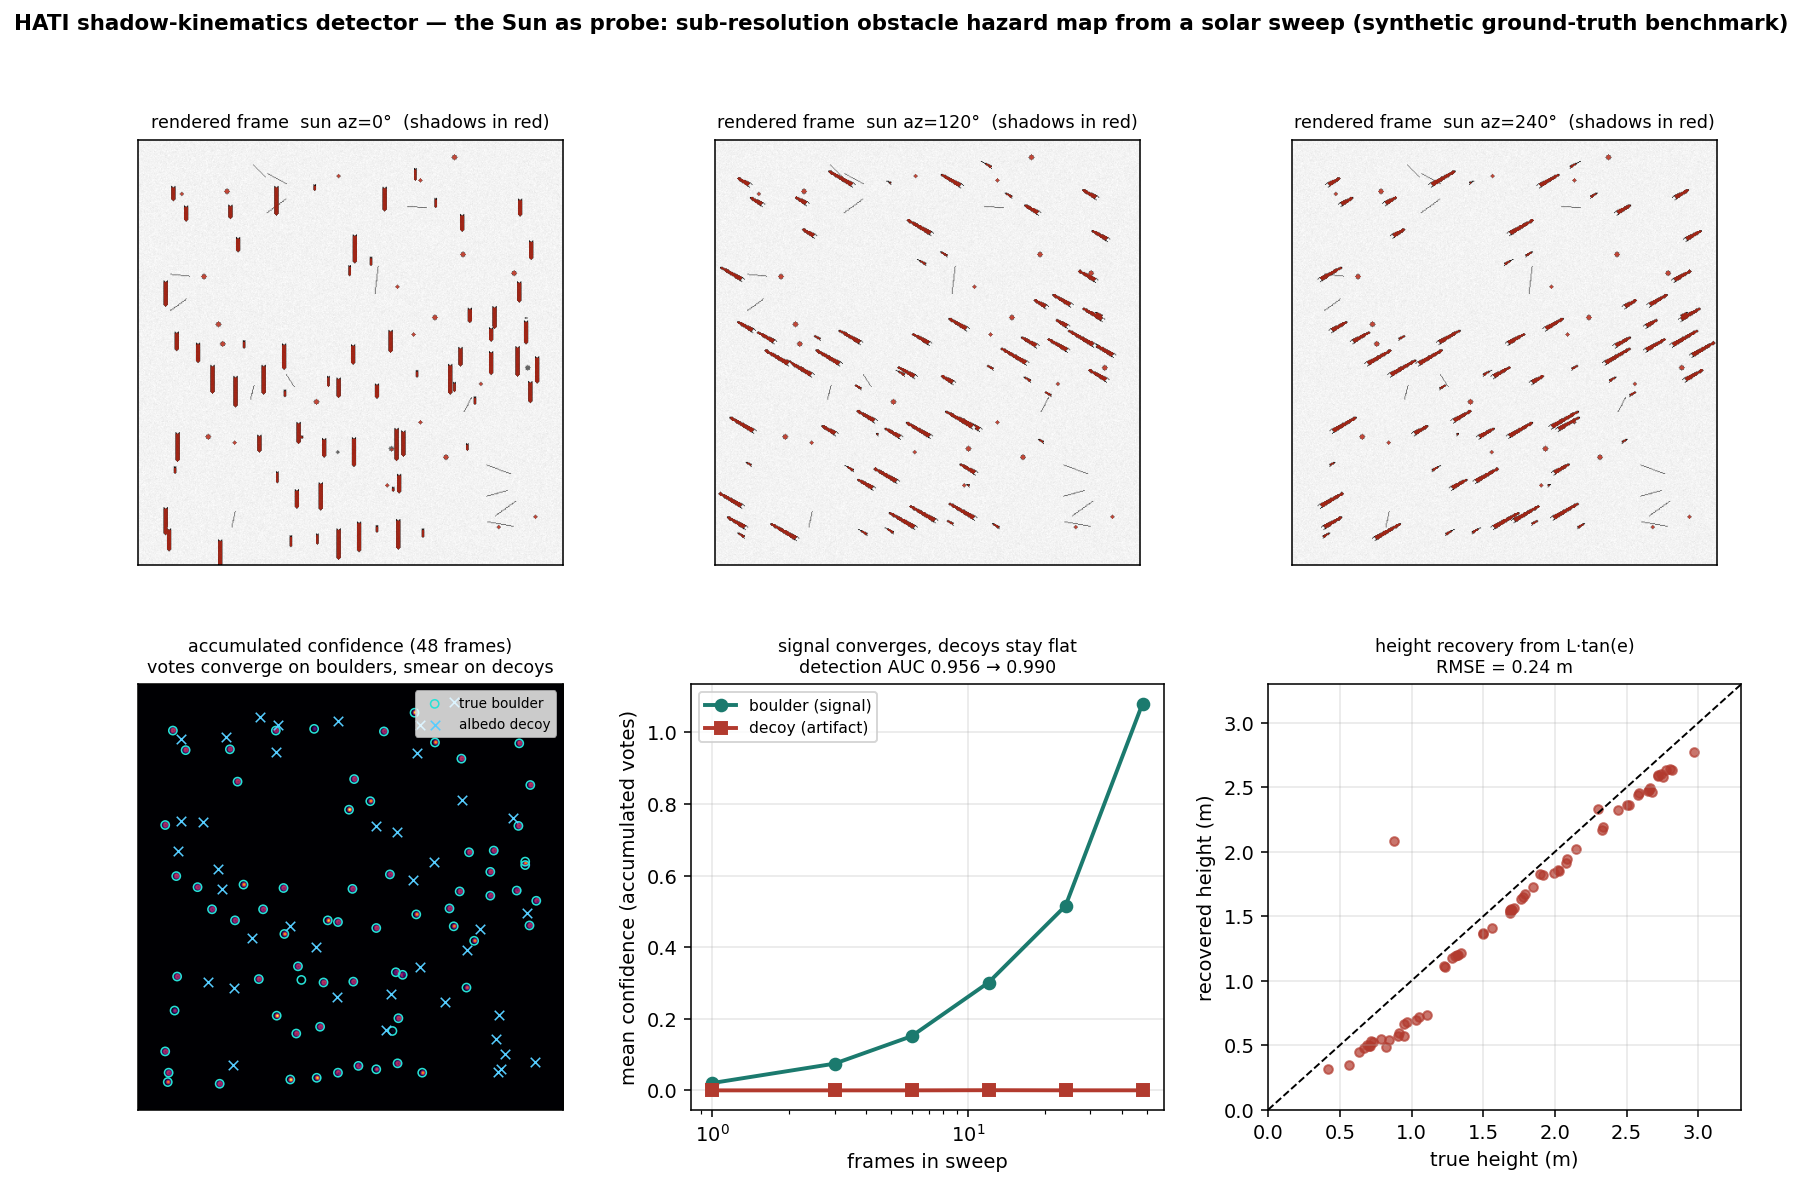
\includegraphics[width=\textwidth]{shadow_kinematics_benchmark.png}
\caption{The Sun as probe, on synthetic ground truth. \textbf{Top:} the same scene rendered
under solar azimuths \ang{0}, \ang{120}, \ang{240}; the cast shadows (red) pivot bodily about
their casters. \textbf{Lower left:} the accumulated confidence map after \num{48} frames ---
votes converge on the true obstacles (cyan rings) and never settle on the albedo decoys (blue
crosses). \textbf{Lower middle:} obstacle confidence (the signal) grows with sweep size while
decoy confidence (the artifact) stays flat at zero. \textbf{Lower right:} height recovered
from $L\tan e$ against the truth, RMS error \SI{0.24}{\meter}.}
\label{fig:bench}
\end{figure}

% =====================================================================
\section{Where this sits in the v2.5 pipeline}

The channel is the sub-resolution complement to the deterministic slope gate. The gate rules
on gross terrain in physical units and transfers between sites; the shadow-kinematics map
rules on the metre-scale obstacles and shallow craters the gate is too coarse to see, which
is precisely the Athena failure class. Its output is an obstacle map with a height attached
to every detection, which feeds a strike probability of the standard Poisson form,
$P=1-\exp(-\lambda A)$, with $\lambda$ the areal density of obstacles above the lander's
clearance and $A$ the footprint area. Because the estimator is geometric and deterministic,
it carries the same audit property as the rest of HATI: every flagged obstacle traces to a
shadow that moved with the Sun in a way a reviewer can replay.

The required data already exist. A query of the NASA Orbital Data Explorer over the Athena
site returns \num{696} LROC narrow-angle frames, \num{525} of them with the Sun above the
horizon, spanning \SIrange{2010}{2024}{} and filling all twelve \ang{30} azimuth sectors ---
an over-determined sweep, because the south pole is one of the most repeatedly imaged places
on the Moon and its Sun circles the horizon at a few degrees' elevation all month.

% =====================================================================
\section{What remains, stated honestly}
\label{sec:limits}

\begin{limitbox}
The benchmark proves the \emph{estimator}, not yet a result on the Moon. Three things stand
between this and a real-data hazard map, and none are hidden.

\emph{Azimuth diversity is mandatory, and the data on hand do not have it.} The three
NOBILE03 orthophotos already co-registered to the site grid were taken within twelve hours,
at solar azimuths of only \ang{173}--\ang{179} and one elevation. They are a single
illumination; on them this method can only denoise, not sense motion. The method needs the
azimuth-spread frames from the \num{525}-frame sweep above.

\emph{Those frames are raw.} Turning archived narrow-angle frames into co-registered
orthophotos is real work --- radiometric calibration, map projection, and sub-pixel
registration to the reference grid --- not a download. The error budget that matters is the
co-registration: a shadow base mislocated by registration jitter blurs the confidence peak
and biases the height. Quantifying that budget on real frames is the first task once they are
ingested.

\emph{The synthetic test is favourable by construction.} Real ground is not flat, real
shadows fall across slopes that bias \cref{eq:shadowlaw}, and real albedo is more varied than
two decoy types. The honest next step is to repeat the benchmark on a real-terrain background
with a measured reflectance, and to fold the local slope --- recoverable from the same
multi-illumination stack by photometric means --- into the height estimate rather than
assuming flat ground.
\end{limitbox}

\noindent
None of these change the conclusion the benchmark does support: given a co-registered solar
sweep, the kinematics of shadows separate metre-scale obstacles from albedo without a
photometric model and measure their heights to a quarter of a metre, well beneath the floor
of any elevation model in hand. Assembling that sweep from the archive, and characterising
the co-registration budget on real frames, is the next development step.

\medskip\hrule\medskip
\noindent\footnotesize\textit{Reproducibility.} The detector and synthetic benchmark are
\texttt{scripts/shadow\_kinematics.py}; the archive query that establishes sweep availability
is \texttt{scripts/solar\_sweep\_query.py}. Both are deterministic given the stated seed and
query box.

\printbibliography

\end{document}
